\section{Monofilare Helixantenne}
Die Helixantenne ist die in der Satellitenkommunikationstechnik die am Weitesten verbreitete Antennenart \cite{HelicalAntennas}. Der Grund hierfür ist die Immunität der zirkularen Polarisation gegenüber Faraday Rotation. Dieses Phänomen findet in der Ionosphäre statt \cite{FaradayRotation} und wurde in (REFERENZ) bereits näher erklärt.

Die Helixantenne hat weiters verschiedene Operationsmodi. Arbeitet die Antenne im Normal-Modus, so zeigt sie ein omnidirektionales Abstrahlverhalten, wobei sie senkrecht zur Achse der Antenne gleichmäßig in alle Richtungen strahlt. Dieser Betriebsmodus wird erreicht, sobald der Umfang einer Windung der Helix im Vergleich zu der Wellenlänge $\lambda=\frac{c}{f}$ klein ist. Der zweite Modus der Wendelantenne ist der Axial-Modus. Befindet sich die Antenne in diesem Betriebsverhalten, so verändert sich die Richtung der Strahlung. Der Großteil der elektromagnetischen Strahlung wird nun entlang der Achse der Spirale abgegeben. Dieser Modus wird erreicht, sobald die Wellenlänge ungefähr gleich groß ist wie der Umfang einer Windung der Spirale. \cite{HelicalAntennas}.

Da die Wendelantenne über eine besonders große Bandbreite verfügt, eignet sie sich gut für den Nachbau. Hierbei sind der Durchmesser sowie die Steigung der Spirale von ausschlaggebender Relevanz für die gewünschte Einsatzfrequenz. Der Durchmesser für eine Wendelantenne im Axial-Modus ist hierbei mit $D=\frac{\lambda}{\pi}$ definiert. Die Stromverteilung auf der Helix ergibt sich folglich wie in Abbildung \ref{fig:CrntDis-Helix} ersichtlich. \cite{HelicalAntennas}.

\begin{figure}[H]
	\centering
	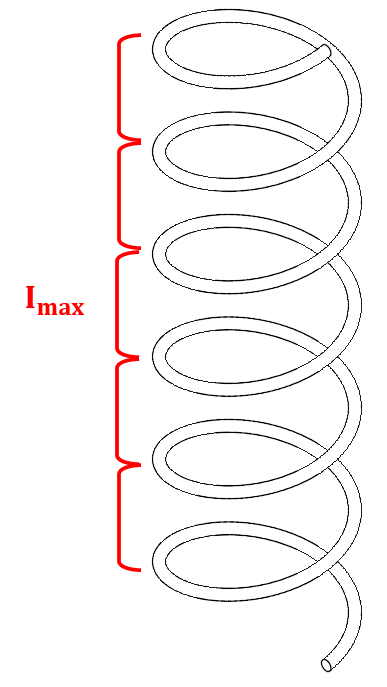
\includegraphics[width=4cm]{../ref/Spirale_Doku}
	\caption{Stromverteilung auf einer Helix-Antenne}
	\label{fig:CrntDis-Helix}
\end{figure}

Die ideale Steigung der Helixantenne befindet sich zwischen den 

\subsection{Vorteile}
Der große Vorteil von Helixantennen besteht darin, dass diese Antennenbauform die einfachste ist, um eine zirkulare Polarisation zu erzielen. Durch eine zirkulare Polarisation, wie bereits in QUERVERWEIS erwähnt, können sowohl horizontal als auch vertikal polarisierte elektromagnetische Wellen empfangen werden.

\subsection{Funktionsweise und charakteristische Eigenschaften}
Dipol/Ringantenne Zusammenhang erklären, zirkulare Polarisation, Zusammenhang mit der Stromverteilung, Erklärung des Abstandes zwischen den Windungen, Durchmesser, Reflektor erklären,

\subsection{Berechnung}
Der Durchmesser der Helix lässt sich mit $D=\frac{\lambda}{\pi}$ berechnen. Dies rührt daher, dass sich mit diesem Durchmesser die Stromverteilung auf der Antenne wie folgt darstellen lässt.